\section{Resultados}

\subsection{Banco de fotos}
\begin{frame}{Construção do banco de fotos}
	\begin{table}
		\centering
		\caption*{Informações sobre o banco de fotos criado, contando quantidade de imagens, se estão presente ou auxentes no Bulário Eletrônico da Anvisa e resolução.}
		\pgfplotstabletypesetfile{../data/banco.dat}
		\caption*{Fonte: Autor.}
	\end{table}
	\begin{itemize}\footnotesize
		\item Baixa resolução, abaixo de \SI{0.92}{\mega\pixel} (HD);
		\item Média resolução, entre \SI{0.92}{\mega\pixel} (HD) e \SI{3.69}{\mega\pixel} (QHD);
		\item Alta resolução, acima de \SI{3.69}{\mega\pixel} (QHD).
	\end{itemize}
\end{frame}


\subsection{Performance}
\begin{frame}{Acurácia para leitura}
	\begin{table}
		\centering
		\caption*{Acurácia geral do sistema, destaque para casos lidos parcial ou corretamente.}
		\resizebox{\textwidth}{!}{%
		\pgfplotstabletypesetfile{../data/geral.dat}
		}
		\caption*{Fonte: Autor.}
	\end{table}
\end{frame}

\begin{frame}
	\begin{figure}
		\centering
		\caption*{Gráfico de acurácia geral do sistema, com \num{1216} itens.}
		\begin{tikzpicture}
    % \pgfsetfillopacity{0.5}

    \begin{axis} %configuração do eixo Y esquerdo e eixo X
    [
        % reverse legend, % inverte a ordem que os items aparecem na legenda
    	legend style={
			% at={($(current bounding box.north)$)},
			at={($(current bounding box.north)+(1cm,0cm)$)},
        	anchor=south,
        	legend columns=3,
        % 	transpose legend,
        	draw=none,
			/tikz/every even column/.append style={column sep=0.5cm}
    	}, % onde exibir
        % axis x line=center,
        % axis y line=center,
        height=.4\textwidth, % altura da região do gráfico
        width=0.8\textwidth, % largura da região do gráfico
        scale only axis, %
        minor grid style={densely dotted}, % estilo da grade secundária
        major grid style={densely dashed}, % estilo da grade principal
        grid style={lightgray}, % cor das grades
        % axis on top, % forçar grade para ficar por cima do gráfico
        %
        %
        % axis y line*=left, % define gráfico para usar eixo esquerdo sem exibir direito
        ylabel={Leitura}, % titulo eixo vertical
        % y tick label style={
        %     /pgf/number format/.cd,
        %     fixed,
        %     % fixed zerofill,
        %     % precision=0, % quantidade de casas depois da virgula
        %     /tikz/.cd
        % },
        % y filter/.expression={y==0 ? NaN : y},
        % scaled y ticks = false,
        % ymode=log,
        % yticklabel={\pgfmathparse{\tick/10^3}\pgfmathprintnumber{\pgfmathresult}}, % fator multiplicativo para valores do eixo
        symbolic y coords={ Correta, Parcial, Incorreta},
        ytick=data,
        % y tick label style={/pgf/number format/1000 sep=}, % Altera marcação de milhar
        y tick label style={rotate=90},
        % yticklabel style={rotate=90},
        %ytick={0,100,200,300, 400, 500, 600, 700, 800}, % lista de valores a serem utilizados no eixo
        % ymin=-5,  ymax=85,  % intervalo de valores no eixo y -> na dúvida, deixe comentado
        %
        % ymajorgrids=true, % exibir grade principal y
        % yminorgrids=true, % exibir grade secundária y
        % minor y tick num=3, % contagem de linhas na grade secundária y
        % ybar,
        %
        %
        xlabel={Casos analisados (\si{\percent})}, % título eixo horizontal
        % xticklabel={\pgfmathparse{\tick*10^3}\pgfmathprintnumber{\pgfmathresult}}, % fator multiplicativo para valores do eixo
        % xmode=log,
        % log ticks with fixed point,
        % x filter/.code=\pgfmathparse{#1 + 6.90775527898214},
        x tick label style={
            /pgf/number format/.cd,
            fixed,
            % fixed zerofill,
            precision=0,
            /tikz/.cd,
            /pgf/number format/use comma
        },
		% symbolic x coords={Nao encontrado, Semelhante, Encontrado},
		% xtick=data,
		% x tick label style={rotate=30,anchor=east},
        xmin=-5,
        xmax=85, % intervalo de valores no eixo x -> na dúvida, deixe comentado
        % scaled x ticks = true,
        %
        xmajorgrids=true, % exibir grade principal x
        xminorgrids=true, % exibir grade secundária x
        minor x tick num=3, % contagem de linhas na grade secundária x
        %
        %
        %
        enlarge y limits=0.25,
        % enlargelimits=0.5,
		xbar stacked,
		bar width = 1.5cm
    ]

    % \addplot[mark=none,red]
    % table[
    %     x=time, % cabeçalho da coluna de dados X no arquivo
    %     y=vin % cabeçalho da coluna de dados Y no arquivo
    % ]
    % {graficos/dados/C.2.2.dat};
    % \addlegendentry{V\textsubscript{in}}

	\addplot[mark=none, draw opacity=0, fill=cmyk_R]
	table[
		y=itens, % cabeçalho da coluna de dados X no arquivo
		x={Não encontrado} % cabeçalho da coluna de dados Y no arquivo
	]
	{../data/acc_geral.dat};
	\addlegendentry{Não encontrado}

	\addplot[mark=none, draw opacity=0, fill=cmyk_G]
	table[
		y=itens, % cabeçalho da coluna de dados X no arquivo
		x=Semelhante % cabeçalho da coluna de dados Y no arquivo
	]
	{../data/acc_geral.dat};
	\addlegendentry{Semelhante}

	\addplot[mark=none, draw opacity=0, fill=cmyk_B]
    table[
        y=itens, % cabeçalho da coluna de dados X no arquivo
        x=Encontrado % cabeçalho da coluna de dados Y no arquivo
    ]
    {../data/acc_geral.dat};
    \addlegendentry{Encontrado}

    \end{axis}
\end{tikzpicture}

		\caption*{Fonte: Autor.}
	\end{figure}
\end{frame}

\begin{frame}{Acurácia para localização}
	\begin{table}
		\centering
		\caption*{Acurácia do sistema somente para casos lidos corretamente, destaque para casas localizados corretamente ou semelhantes.}
		\resizebox{\textwidth}{!}{%
		\pgfplotstabletypesetfile{../data/lido.dat}
		}
		% \medskip
		\caption*{Fonte: Autor.}
	\end{table}
\end{frame}

\begin{frame}
	\begin{figure}
		\caption*{Gráfico de acurácia do sistema somente para casos lidos corretamente, com \num{975} itens.}
		\centering
		\begin{tikzpicture}
    % \pgfsetfillopacity{0.5}

    \begin{axis} %configuração do eixo Y esquerdo e eixo X
    [
        reverse legend, % inverte a ordem que os items aparecem na legenda
    	legend style={
			% at={($(current bounding box.north)$)},
			at={($(current bounding box.north)+(1cm,0cm)$)},
        	anchor=south,
        	legend columns=3,
        % 	transpose legend,
        	draw=none,
			/tikz/every even column/.append style={column sep=0.5cm}
    	}, % onde exibir
        % axis x line=center,
        % axis y line=center,
        height=.4\textwidth, % altura da região do gráfico
        width=0.8\textwidth, % largura da região do gráfico
        scale only axis, %
        minor grid style={densely dotted}, % estilo da grade secundária
        major grid style={densely dashed}, % estilo da grade principal
        grid style={lightgray}, % cor das grades
        % axis on top, % forçar grade para ficar por cima do gráfico
        %
        %
        % axis y line*=left, % define gráfico para usar eixo esquerdo sem exibir direito
        ylabel={Casos analisados (\si{\percent})}, % titulo eixo vertical
        y tick label style={
            /pgf/number format/.cd,
            fixed,
            % fixed zerofill,
            % precision=0, % quantidade de casas depois da virgula
            /tikz/.cd
        },
        % y filter/.expression={y==0 ? NaN : y},
        % scaled y ticks = false,
        % ymode=log,
        % yticklabel={\pgfmathparse{\tick/10^3}\pgfmathprintnumber{\pgfmathresult}}, % fator multiplicativo para valores do eixo
        % symbolic y coords={ Correta, Parcial, Incorreta},
        % ytick=data,
        y tick label style={/pgf/number format/1000 sep=}, % Altera marcação de milhar
        % y tick label style={rotate=60,anchor=east},
        % yticklabel style={rotate=90},
        %ytick={0,100,200,300, 400, 500, 600, 700, 800}, % lista de valores a serem utilizados no eixo
        ymin=-5,
		ymax=90,  % intervalo de valores no eixo y -> na dúvida, deixe comentado
        %
        ymajorgrids=true, % exibir grade principal y
        yminorgrids=true, % exibir grade secundária y
        minor y tick num=3, % contagem de linhas na grade secundária y
        % ybar,
        %
        %
        xlabel={Localização}, % título eixo horizontal
        % xticklabel={\pgfmathparse{\tick*10^3}\pgfmathprintnumber{\pgfmathresult}}, % fator multiplicativo para valores do eixo
        % xmode=log,
        % log ticks with fixed point,
        % x filter/.code=\pgfmathparse{#1 + 6.90775527898214},
        % x tick label style={
        %     /pgf/number format/.cd,
        %     fixed,
        %     % fixed zerofill,
        %     precision=0,
        %     /tikz/.cd,
        %     /pgf/number format/use comma
        % },
		symbolic x coords={Não encontrado, Semelhante, Encontrado},
		xtick=data,
		% x tick label style={rotate=15,anchor=north east},
        % xmin=-5,
        % xmax=50, % intervalo de valores no eixo x -> na dúvida, deixe comentado
        % scaled x ticks = true,
        %
        % xmajorgrids=true, % exibir grade principal x
        % xminorgrids=true, % exibir grade secundária x
        % minor x tick num=9, % contagem de linhas na grade secundária x
        %
        %
        %
        % enlarge y limits=0.25,
        % enlargelimits=0.5,
        enlarge x limits=0.25,
		ybar stacked,
		bar width = 1.5cm
    ]

    % \addplot[mark=none,red]
    % table[
    %     x=time, % cabeçalho da coluna de dados X no arquivo
    %     y=vin % cabeçalho da coluna de dados Y no arquivo
    % ]
    % {graficos/dados/C.2.2.dat};
    % \addlegendentry{V\textsubscript{in}}

	\addplot[mark=none, draw opacity=0, fill=cmyk_C]
    table[
        x=itens, % cabeçalho da coluna de dados X no arquivo
        y=Leitura correta % cabeçalho da coluna de dados Y no arquivo
    ]
    {../data/acc_lido.dat};
    \addlegendentry{Leitura correta}

	\addplot[mark=none, draw opacity=0, fill=cmyk_M]
	table[
		x=itens, % cabeçalho da coluna de dados X no arquivo
		y=Leitura parcial % cabeçalho da coluna de dados Y no arquivo
	]
	{../data/acc_lido.dat};
	\addlegendentry{Leitura parcial}

	% \addplot[mark=none, draw opacity=0, fill=cmyk_Y]
	% table[
	% 	x=itens, % cabeçalho da coluna de dados X no arquivo
	% 	y={Não encontrado} % cabeçalho da coluna de dados Y no arquivo
	% ]
	% {../data/acc_geral.dat};
	% \addlegendentry{Não encontrado}

    \end{axis}
\end{tikzpicture}

		\caption*{Fonte: Autor.}
	\end{figure}
\end{frame}

\begin{frame}{Sem versões alternativas}
	\begin{table}
		\centering
		\caption*{Acurácia geral do sistema sem versões alternativas de imagem e acurácia somente para casos lidos corretamente.}
		\resizebox{\textwidth}{!}{%
		\pgfplotstabletypesetfile{../data/geral_raw.dat}
		}
		\\\vspace{\floatsep}
		\resizebox{\textwidth}{!}{%
		\pgfplotstabletypesetfile{../data/lido_raw.dat}
		}
		% \medskip
		\caption*{Fonte: Autor.}
	\end{table}
\end{frame}

\subsection{Problemas}
\begin{frame}{Problemas encontrados}
	\begin{itemize}
		\item Falhas de acesso;
		\item Orientação de texto;
		\item Reflexos na imagem;
		\item Obstruções na embalagem.
	\end{itemize}
\end{frame}

\begin{frame}{Falhas de acesso}
	\begin{figure}
	    \centering
	    \caption*{Sistema tentando acessar o Bulário Eletrônico, fora do horário comercial.}
	    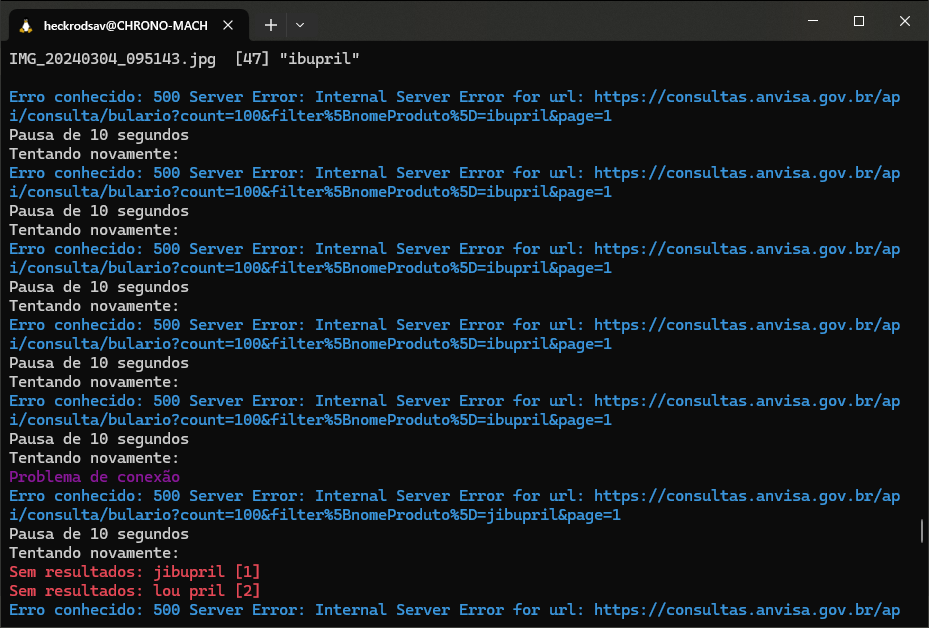
\includegraphics[height=0.7\textheight]{../pictures/Anvisa_domingo.png}
	    \caption*{Fonte: Autor, captura realizada em 2024-03-13.}
	\end{figure}
\end{frame}

\begin{frame}
	\begin{figure}
	    \centering
	    \caption*{Bulário Eletrônico com erro 404, fora do horário comercial.}
	    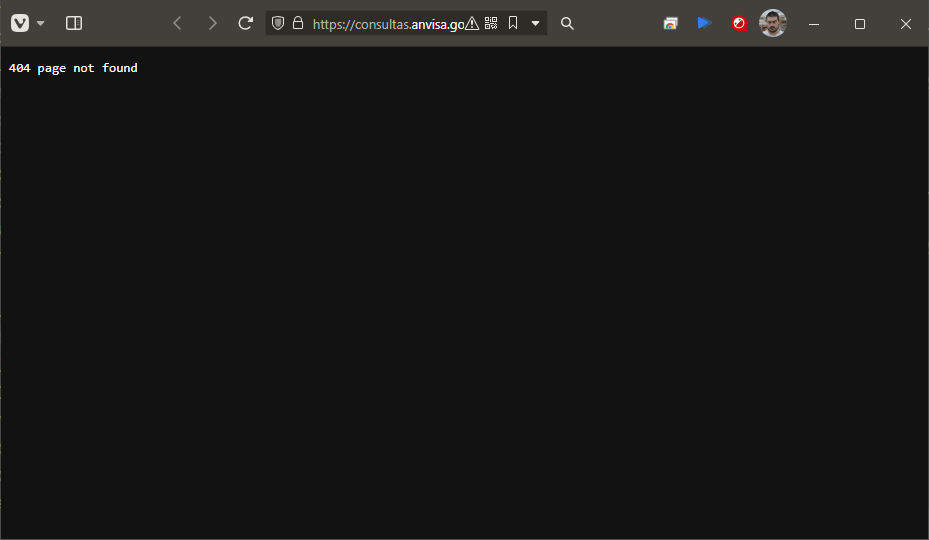
\includegraphics[height=0.7\textheight]{../pictures/Anvisa_error_404.png}
	    \caption*{Fonte: Autor, captura realizada em 2024-03-13.}
	\end{figure}
\end{frame}

\begin{frame}
	\begin{figure}
	    \centering
	    \caption*{Erro no servidor do Bulário Eletrônico, fora do horário comercial.}
	    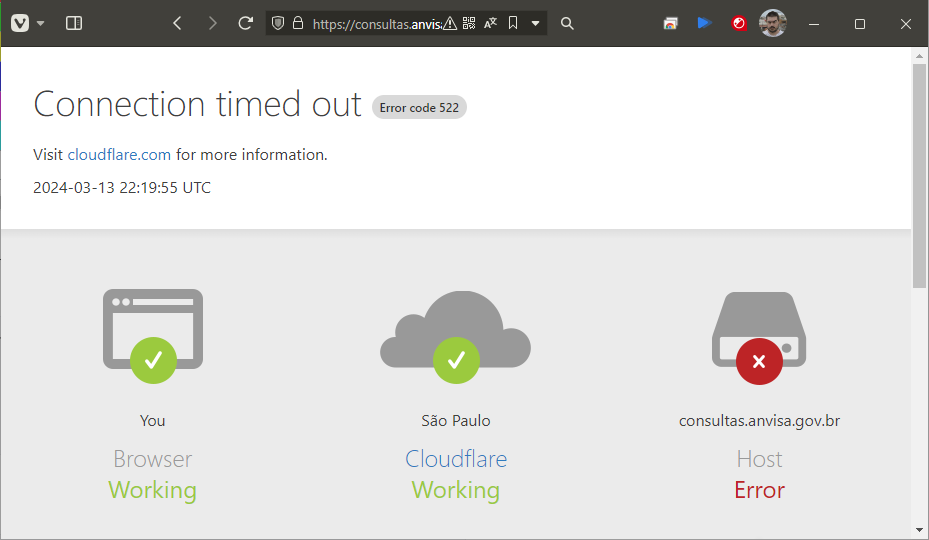
\includegraphics[height=0.7\textheight]{../pictures/Anvisa_error_timeout.png}
	    \caption*{Fonte: Autor, captura realizada em 2024-03-13.}
	\end{figure}
\end{frame}

\begin{frame}
	\begin{figure}
	    \centering
	    \caption*{Erro interno no servidor do Bulário Eletrônico, dentro do horário comercial.}
	    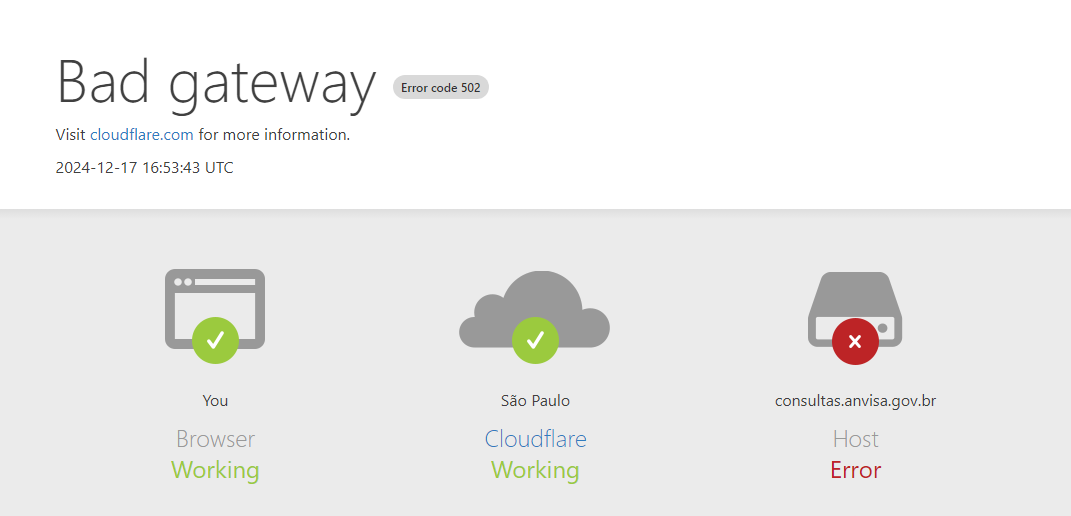
\includegraphics[keepaspectratio, width=0.95\textwidth, height=0.7\textheight]{../pictures/2024-12-17 13.55.09 consultas.anvisa.gov.br 097b2055395f.png}
	    \caption*{Fonte: Autor, captura realizada em 2024-12-17.}
	\end{figure}
\end{frame}

\begin{frame}{Orientação do texto}
	\centering
	\captionof*{figure}{Fotos de medicamento com diferentes orientações de texto.}
	\begin{columns}
		\begin{column}{0.5\textwidth}
			\centering
			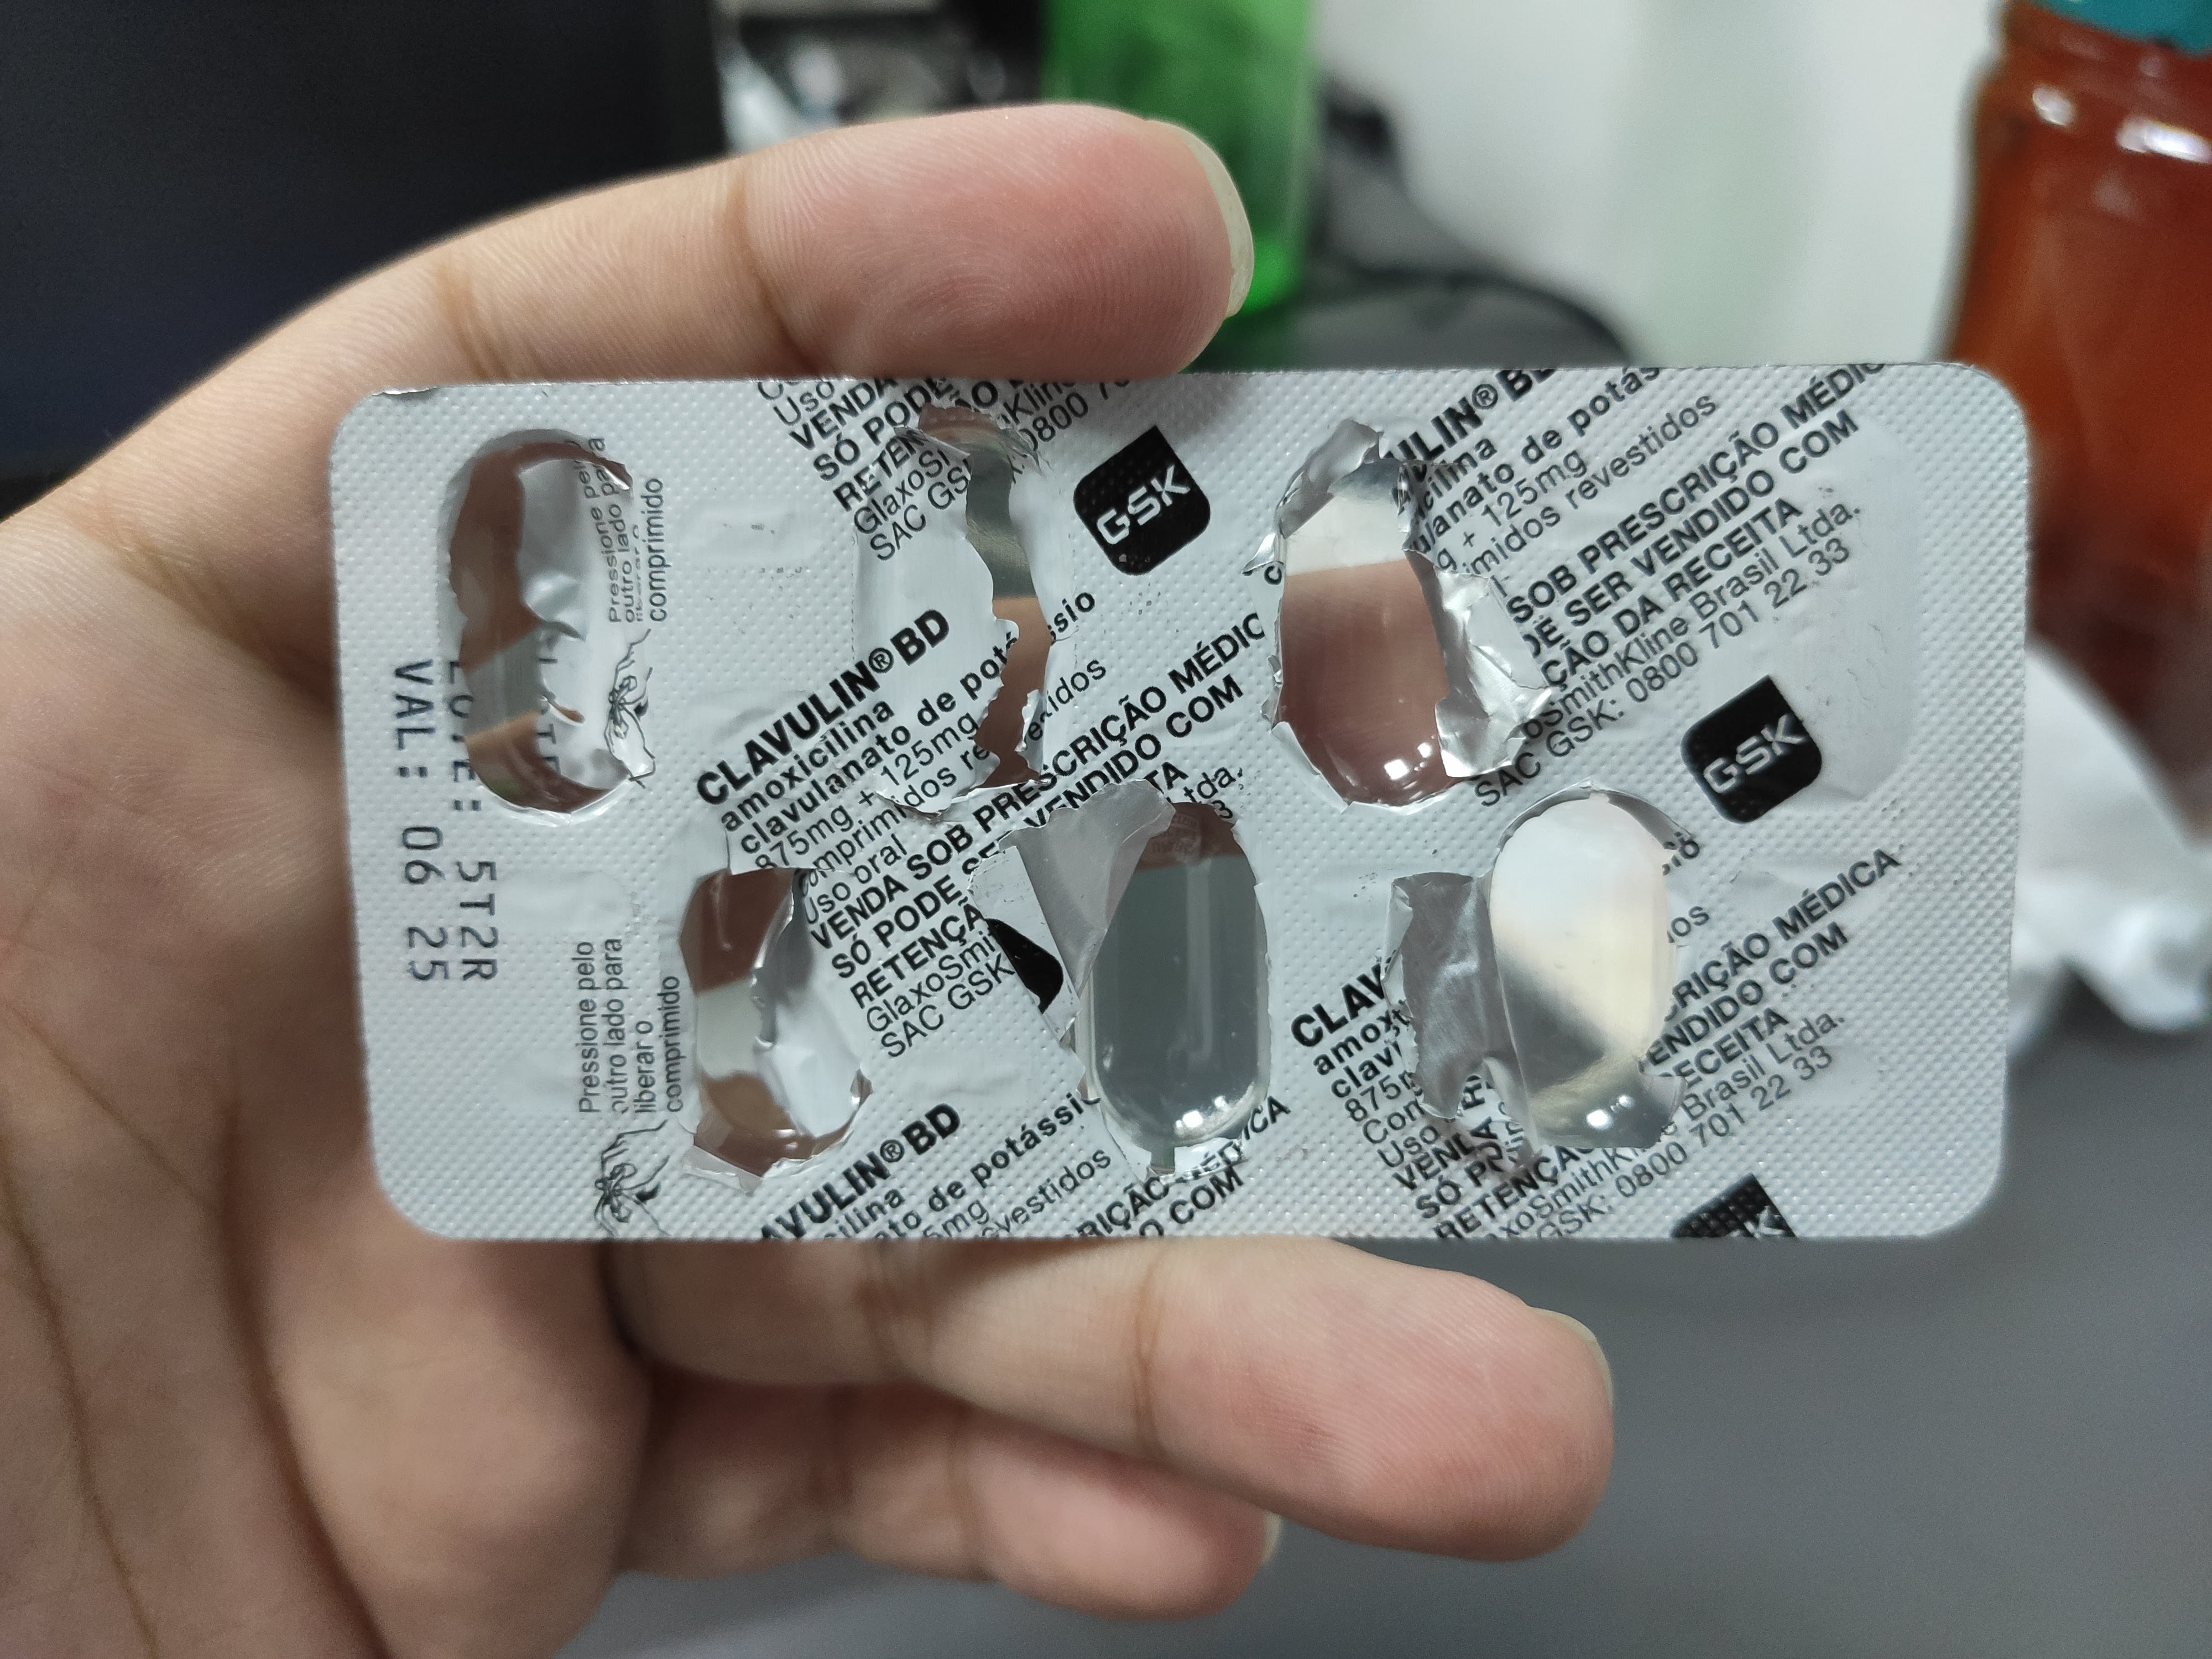
\includegraphics[width=\textwidth]{../pictures/IMG_20240229_162005.jpg}
			\captionof*{figure}{Diagonal à horizontal.}
		\end{column}
		\begin{column}{0.5\textwidth}
			\centering
			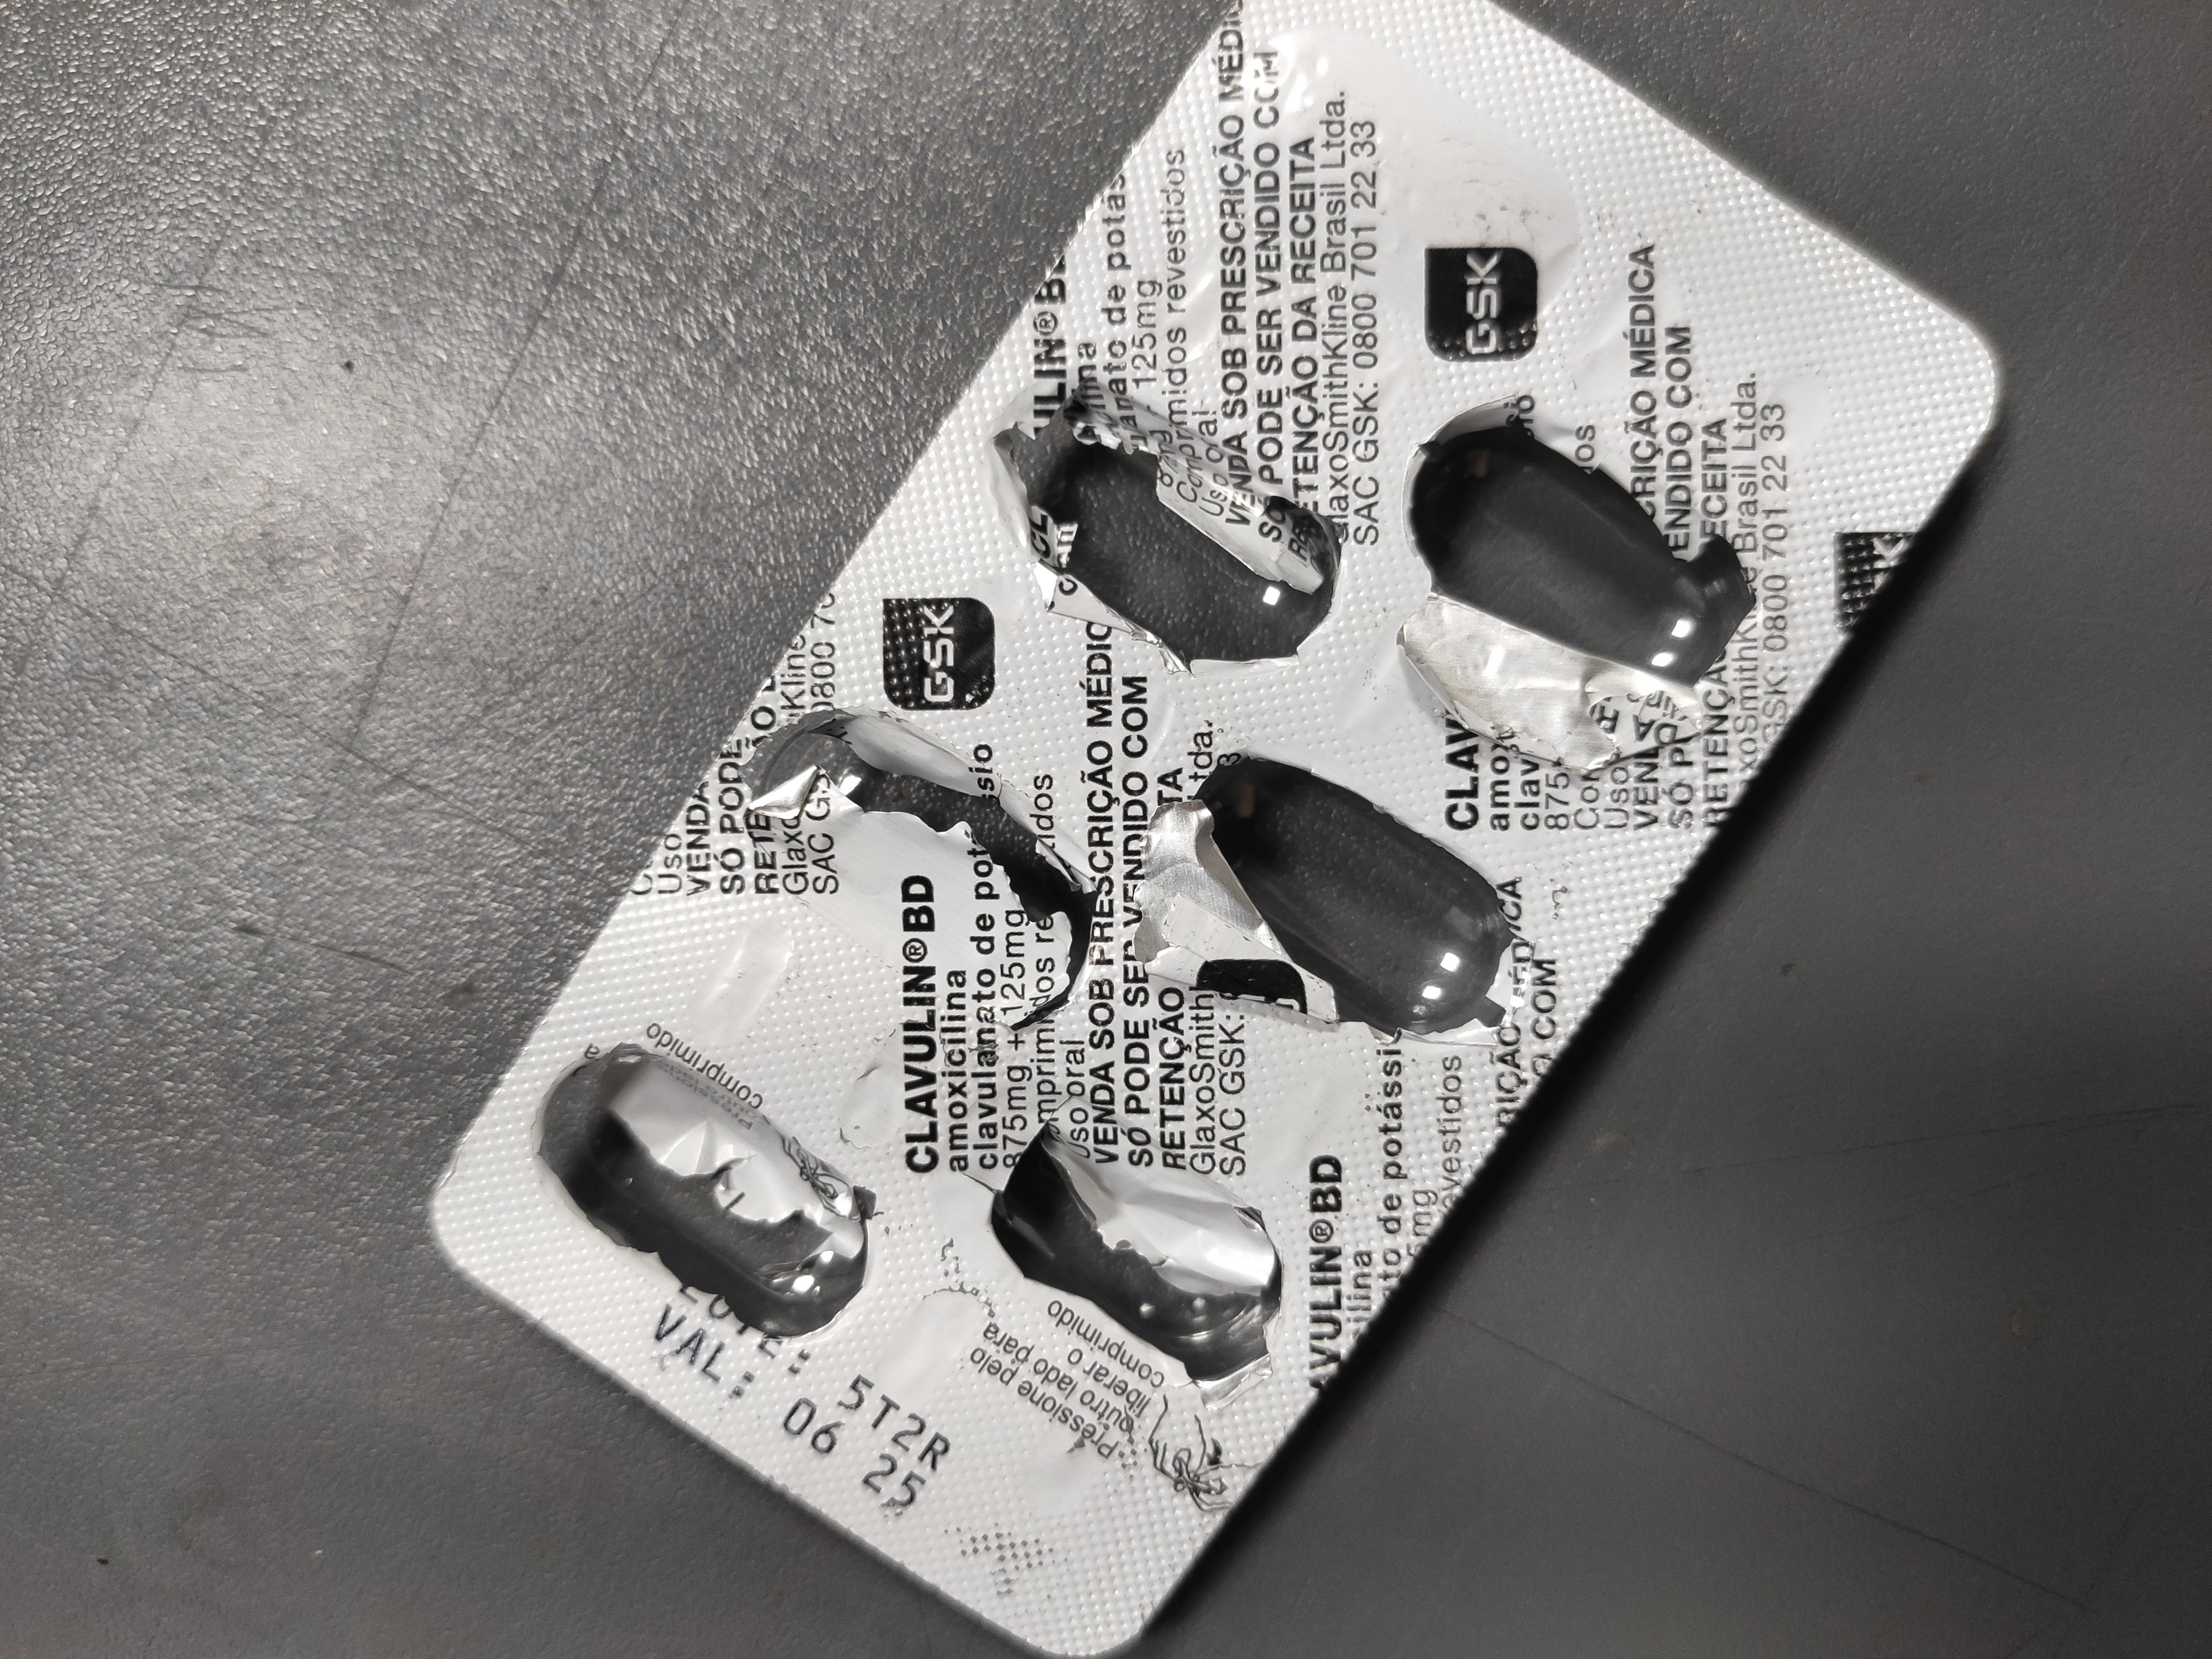
\includegraphics[width=0.9\textwidth, angle=-90]{../pictures/IMG_20240307_185809.jpg}
			\captionof*{figure}{Paralela à horizontal.}
		\end{column}
	\end{columns}
	\captionof*{figure}{Fonte: Autor.}
\end{frame}

\begin{frame}{Reflexos na imagem}
	\centering
	\captionof*{figure}{Fotos de medicamento com e sem reflexos sobre texto de interesse.}
	\begin{columns}
		\begin{column}{0.5\textwidth}
			\centering
			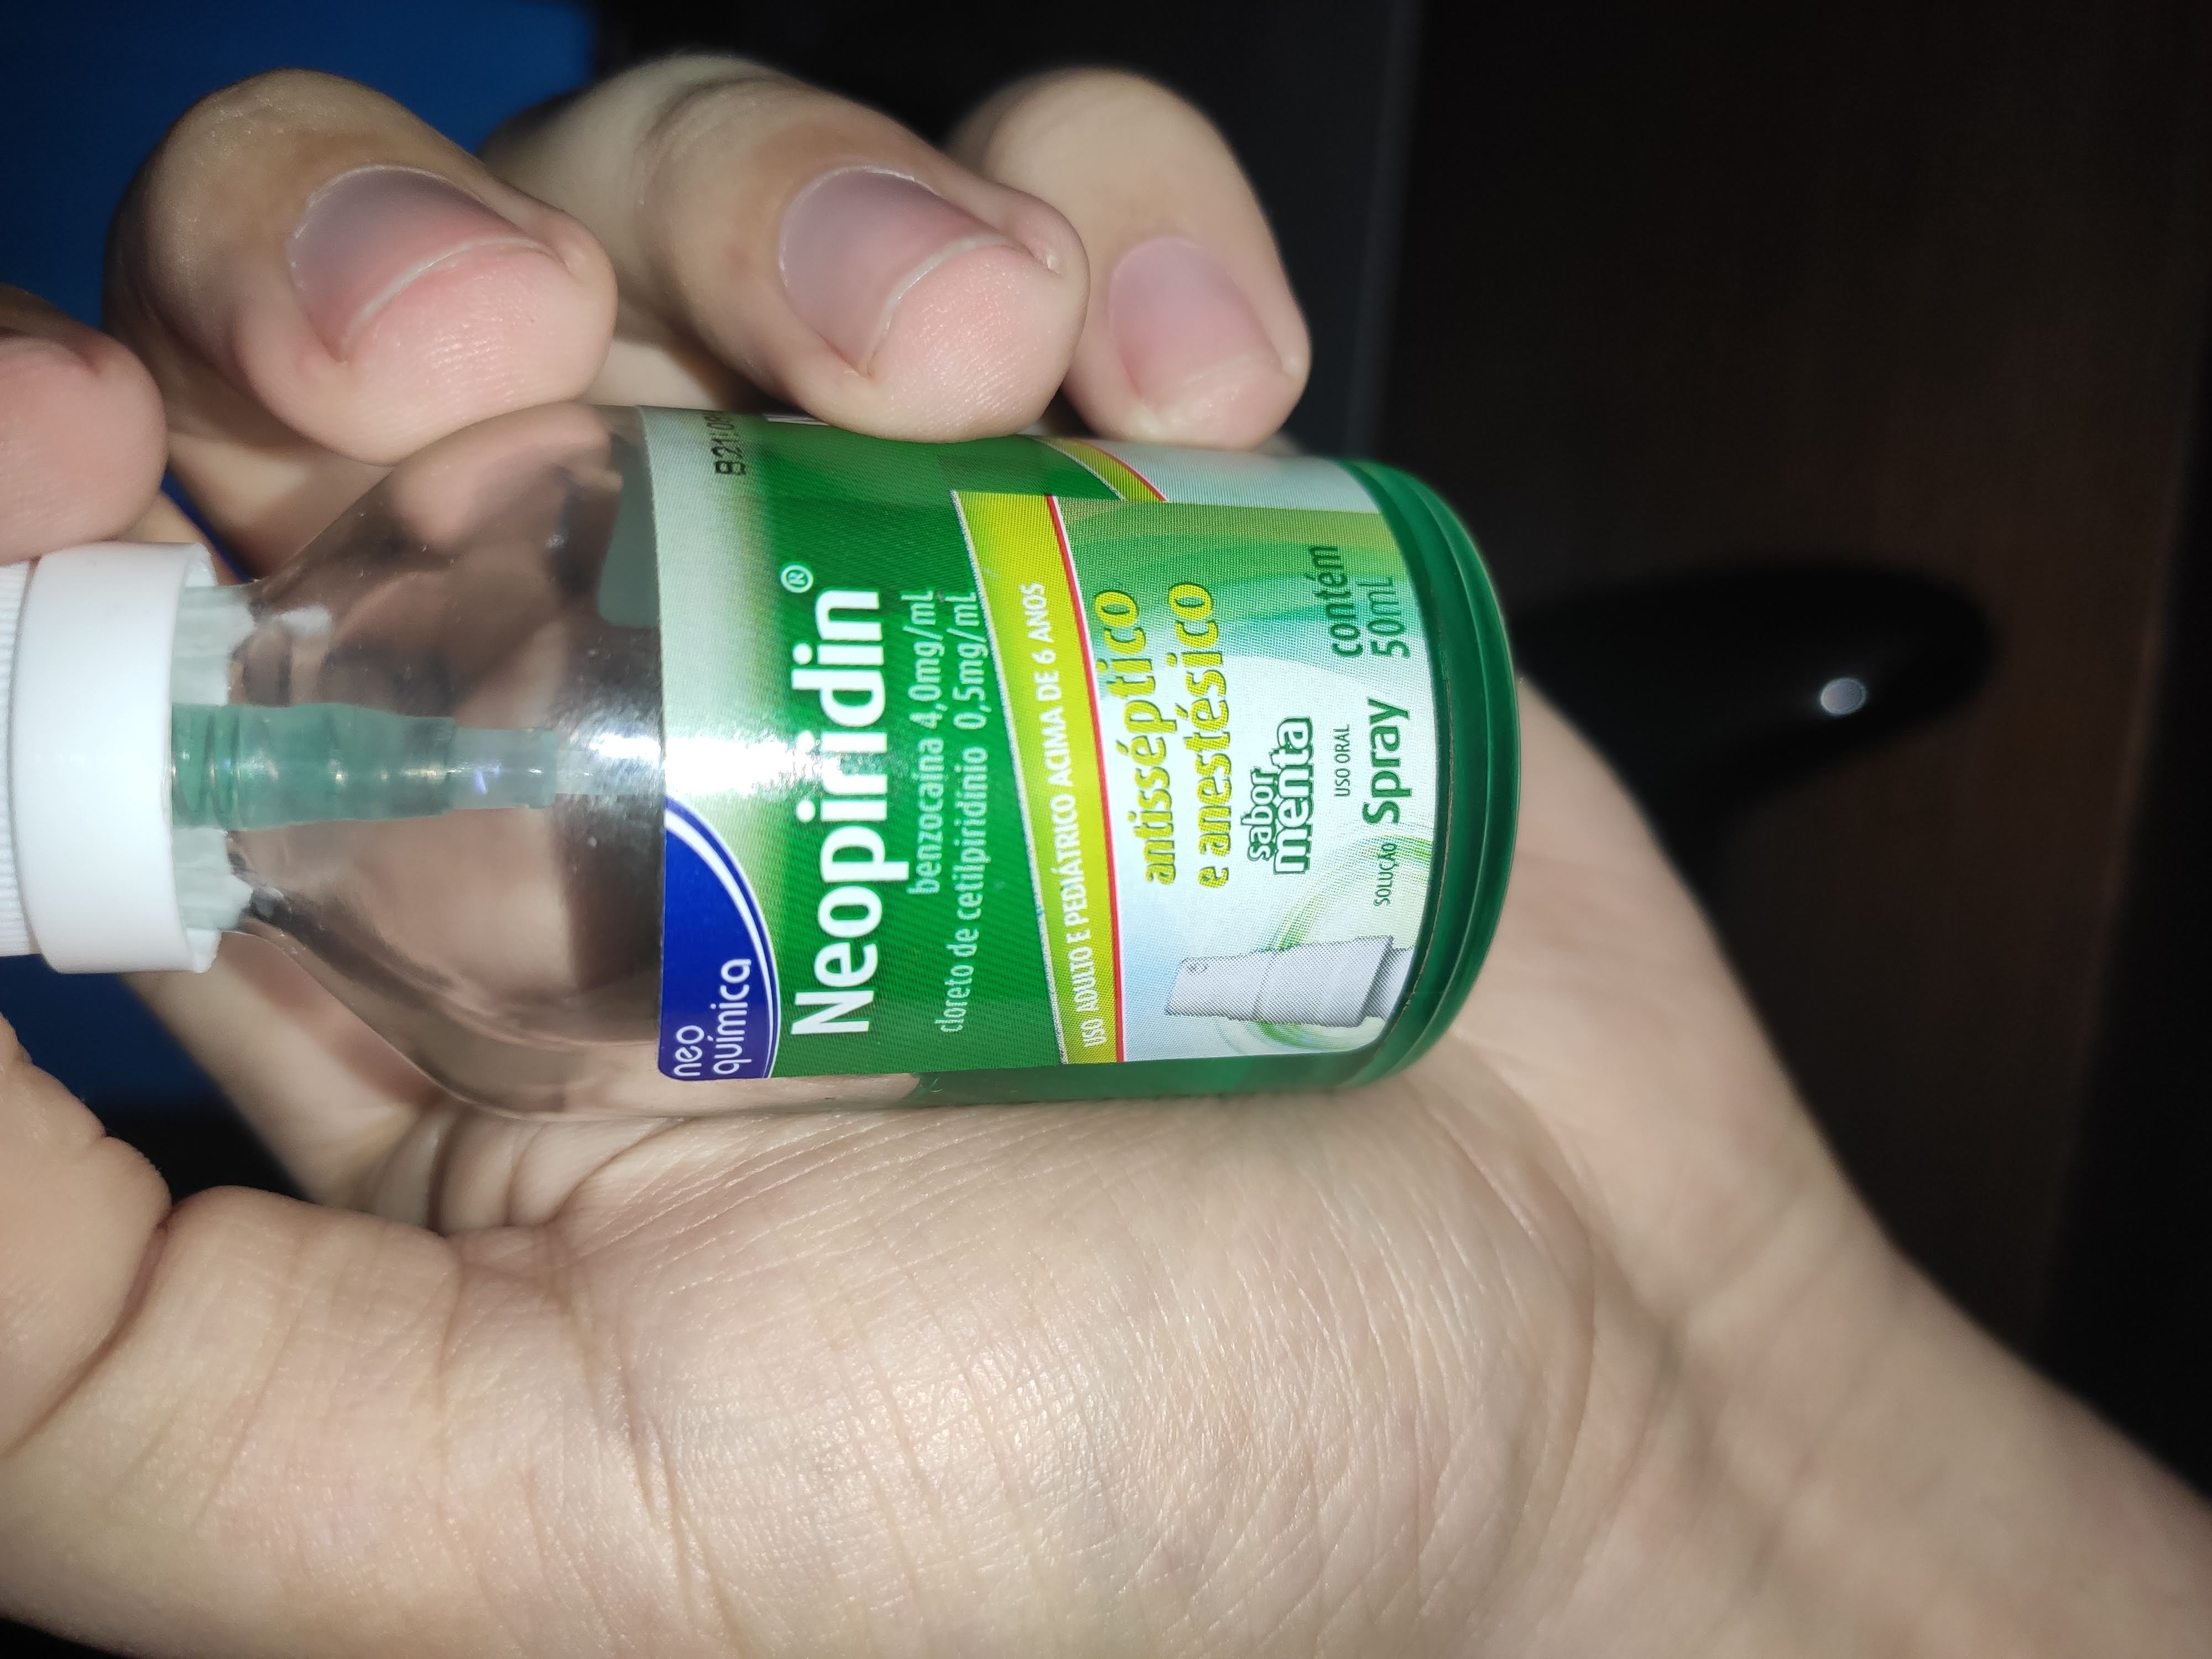
\includegraphics[keepaspectratio, width=0.9\textwidth, angle=-90]{../pictures/IMG_20220908_191849.jpg}
			\captionof*{figure}{Com reflexo.}
		\end{column}
		\begin{column}{0.5\textwidth}
			\centering
			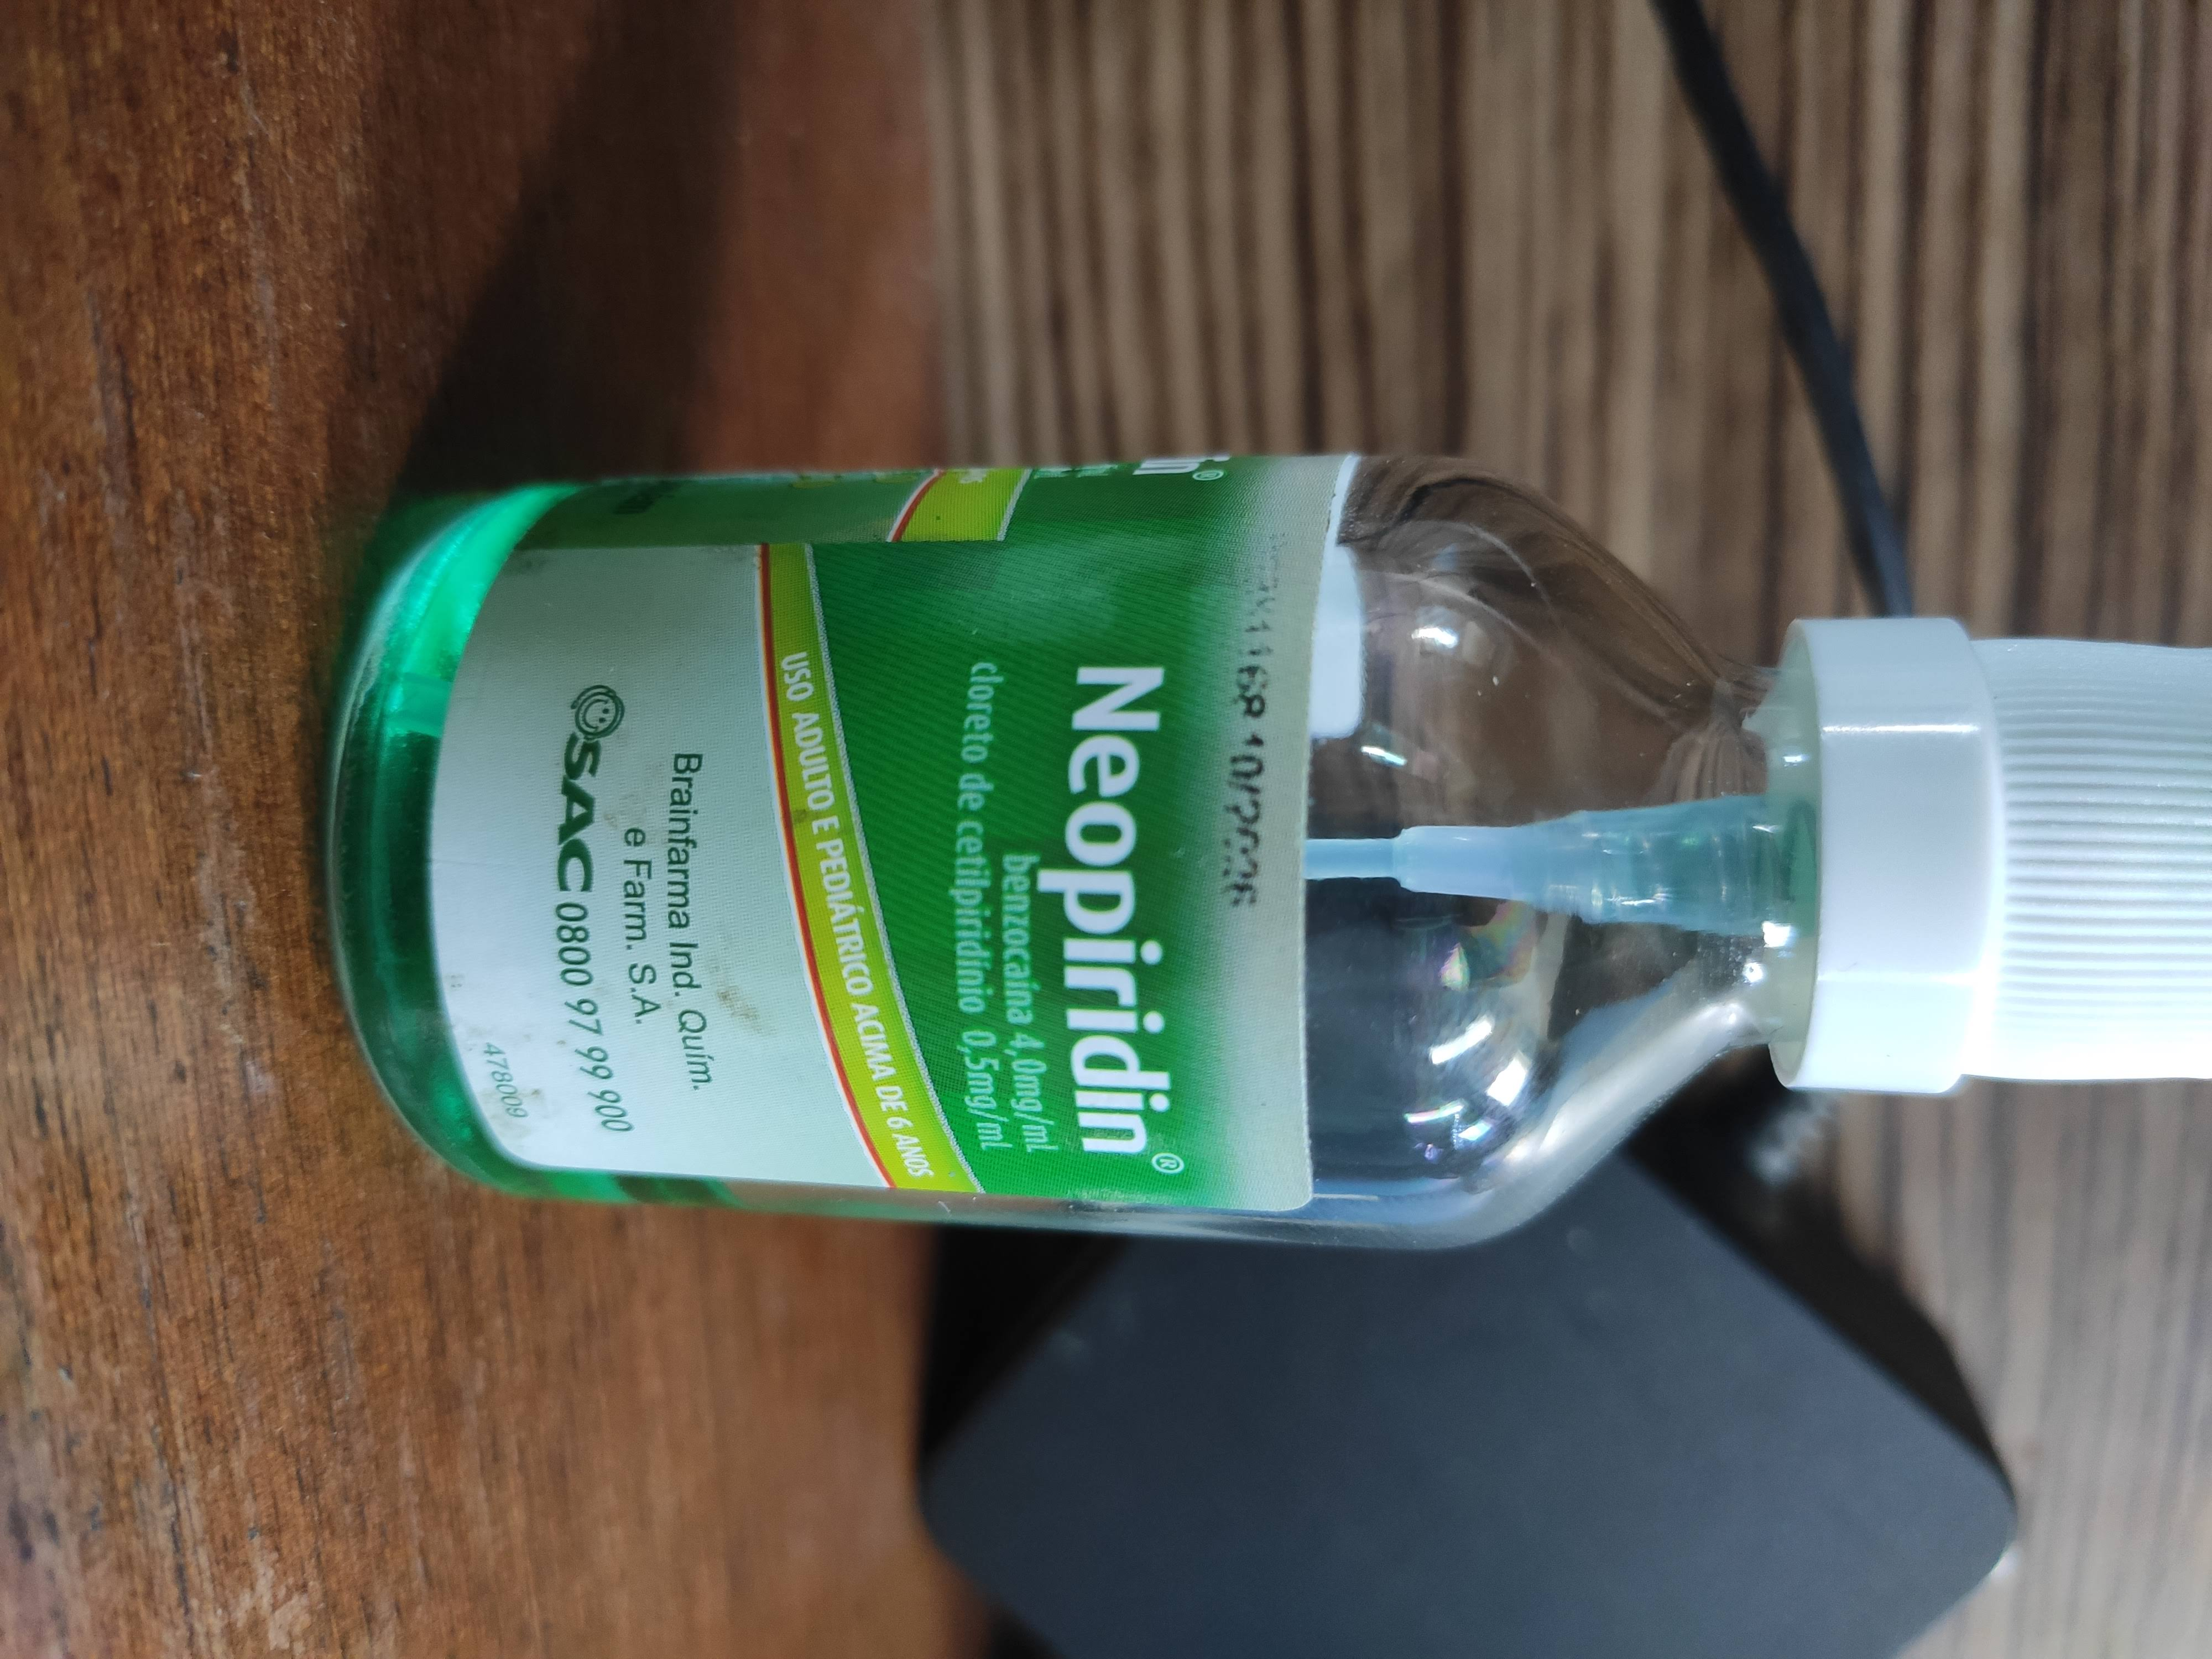
\includegraphics[keepaspectratio, width=0.9\textwidth, angle=90]{../pictures/IMG_20240301_105852.jpg}
			\captionof*{figure}{Sem reflexo.}
		\end{column}
	\end{columns}
	\captionof*{figure}{Fonte: Autor.}
\end{frame}

\begin{frame}{Obstruções na embalagem}
	\centering
	\captionof*{figure}{Fotos de medicamento com e sem rasuras na região do texto..}
	\begin{columns}
		\begin{column}{0.5\textwidth}
			\centering
			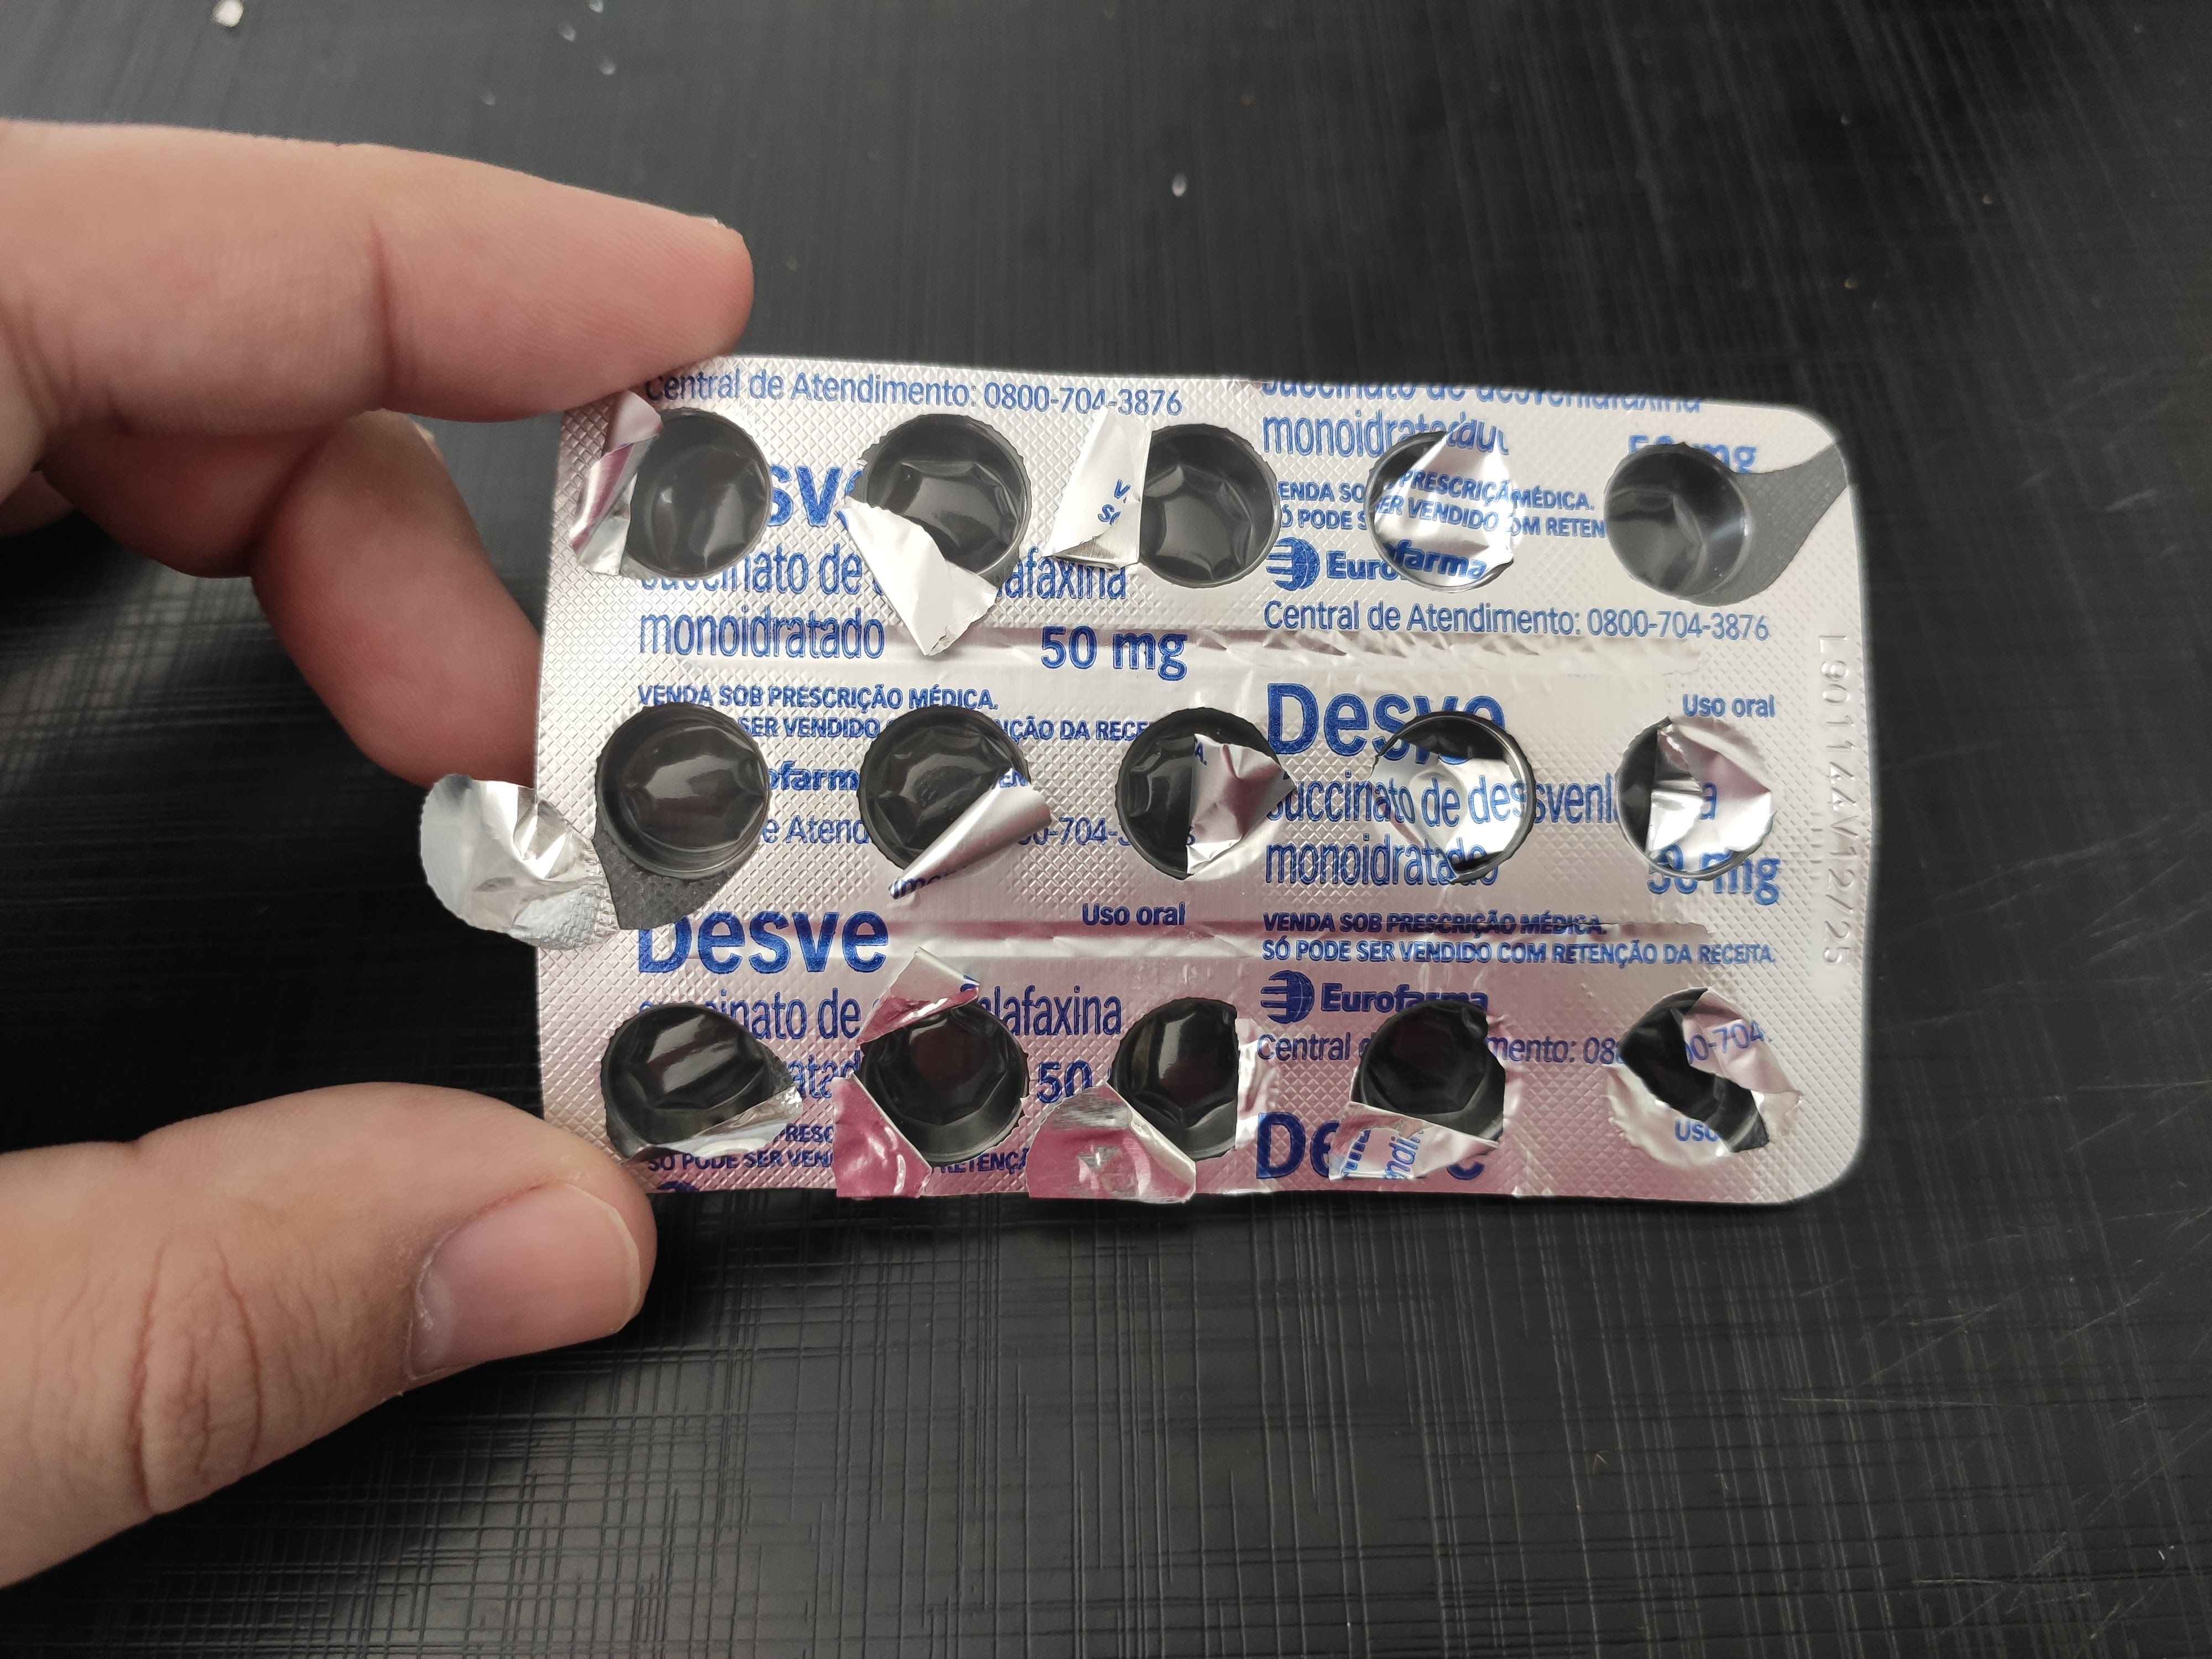
\includegraphics[width=\textwidth]{../pictures/IMG_20240725_110209.jpg}
			\captionof*{figure}{Texto partido.}
		\end{column}
		\begin{column}{0.5\textwidth}
			\centering
			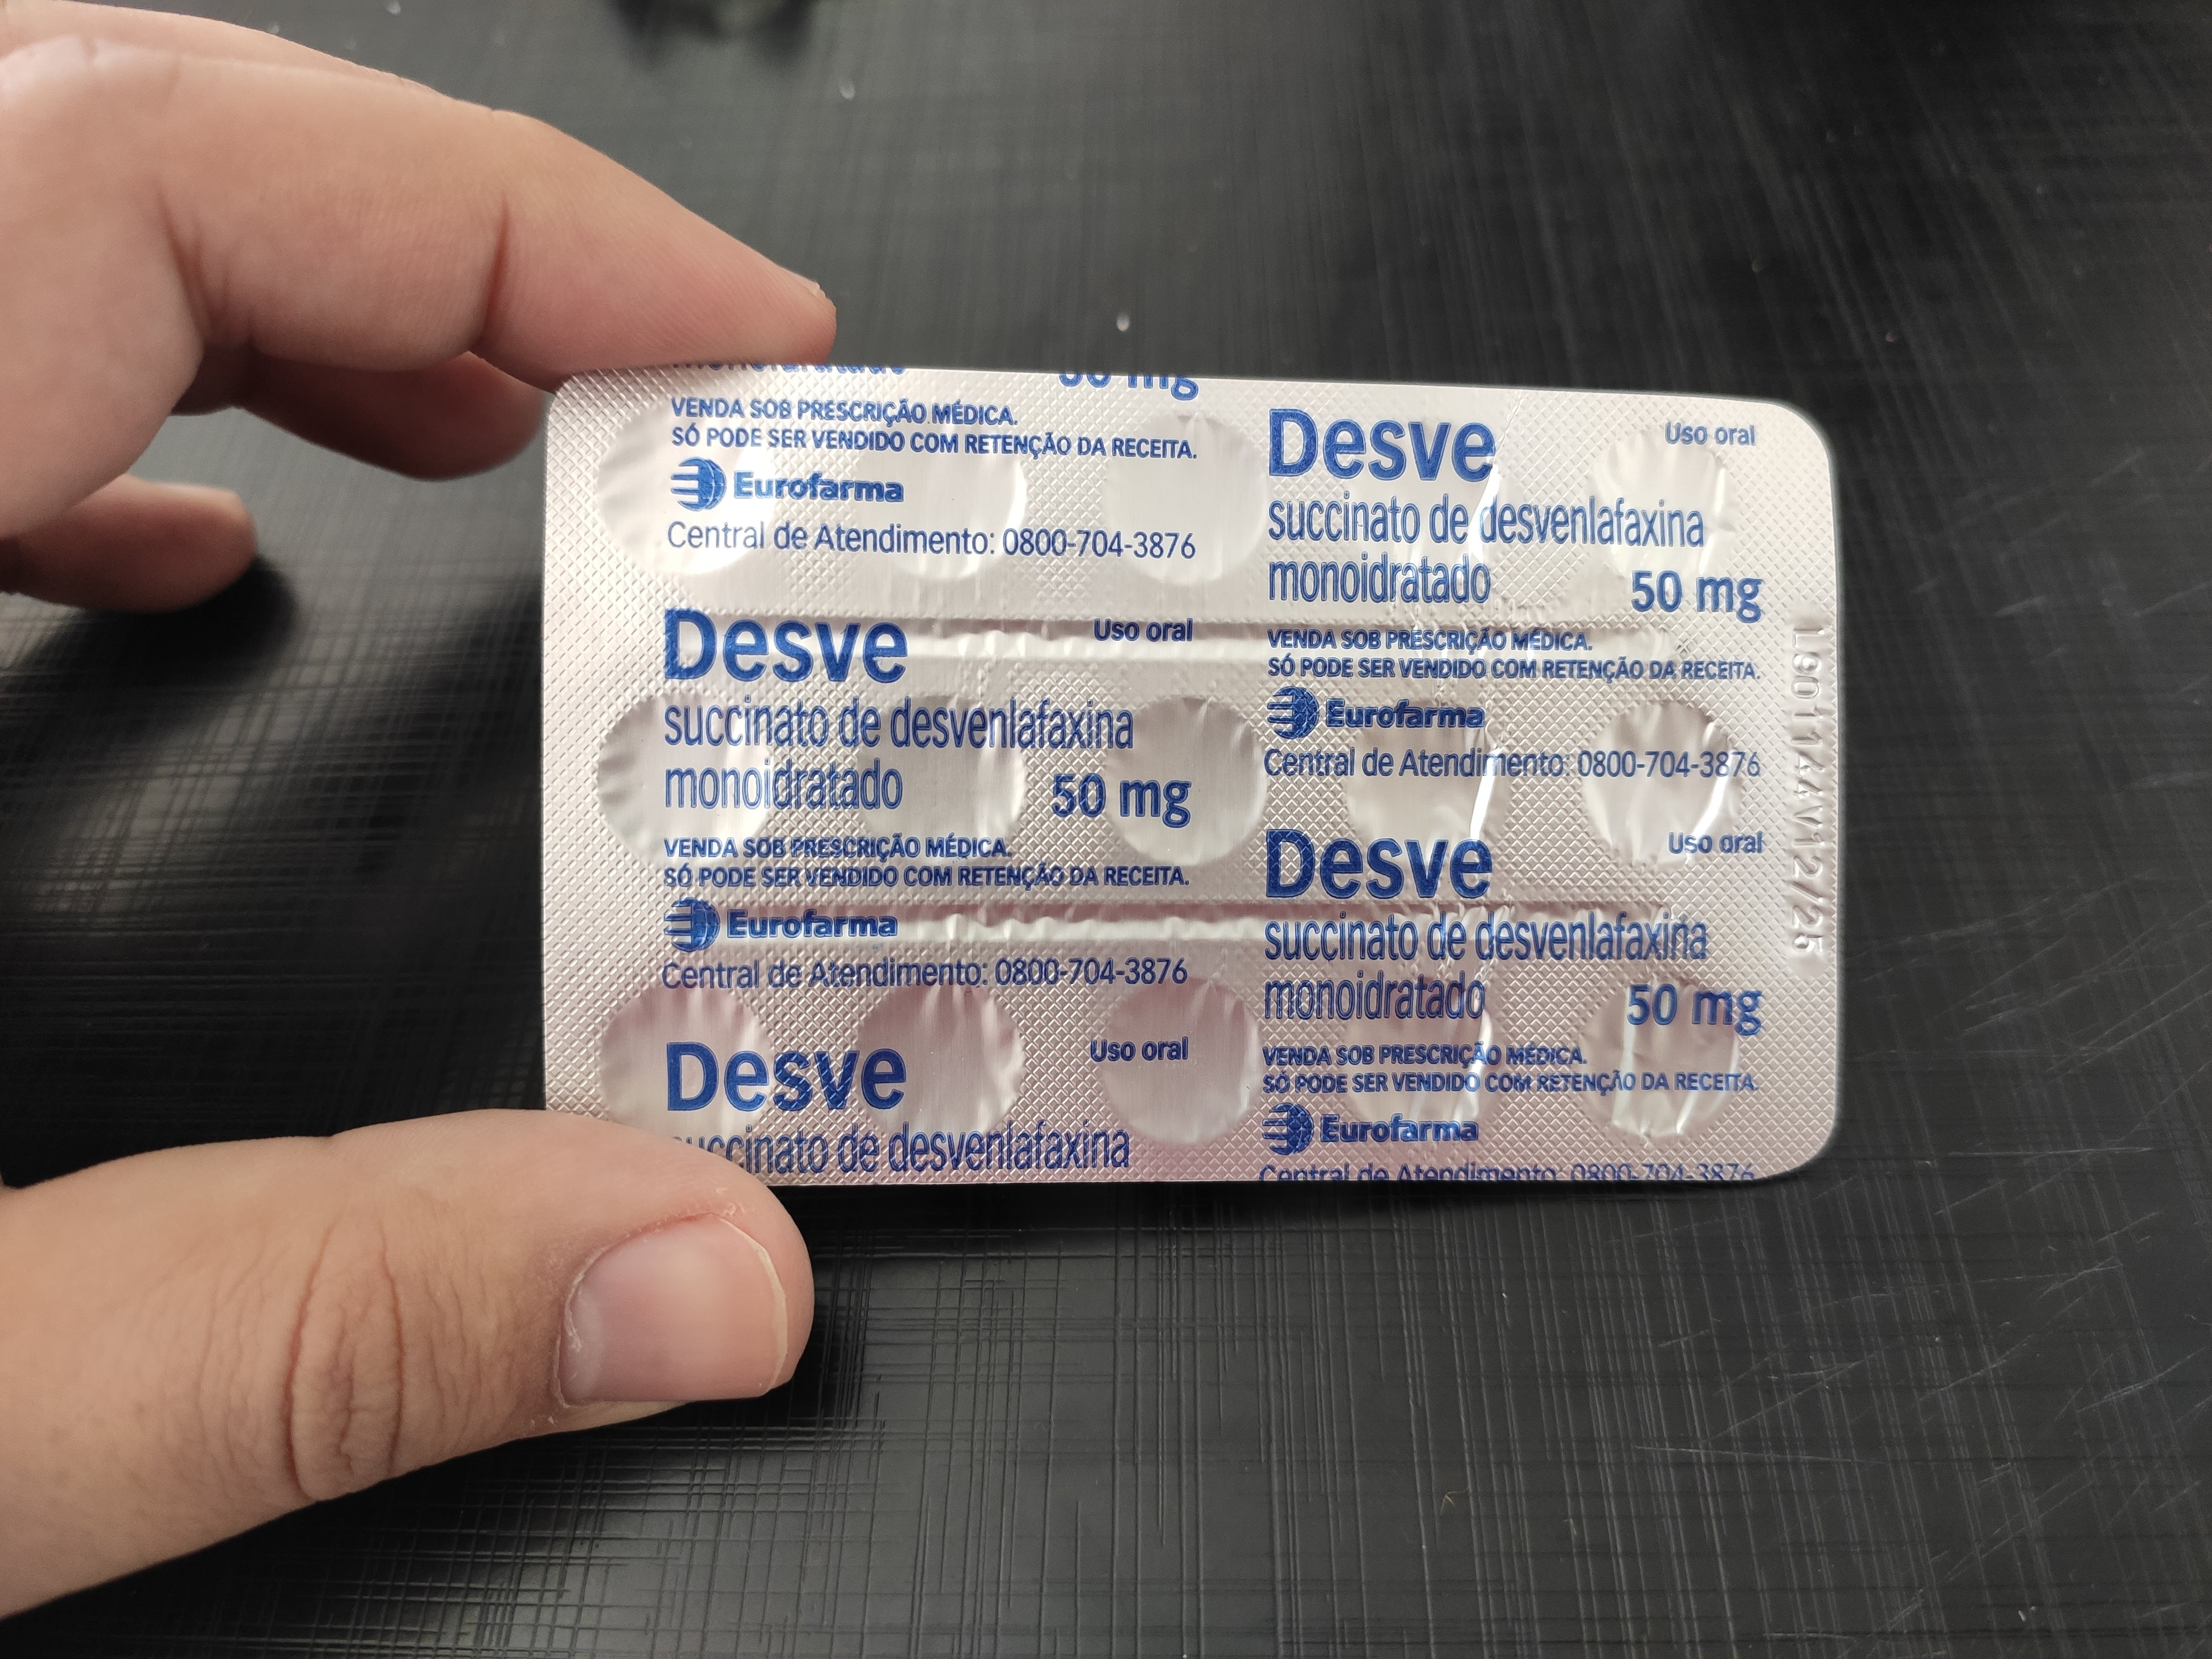
\includegraphics[width=\textwidth]{../pictures/IMG_20240725_110238.jpg}
			\captionof*{figure}{Texto inteiro.}
		\end{column}
	\end{columns}
	\captionof*{figure}{Fonte: Autor.}
\end{frame}
